% !TeX spellcheck = cs_CZ

\documentclass[a4paper]{article}
\usepackage[english]{babel}
\usepackage[utf8x]{inputenc}
\usepackage[T1]{fontenc}
\usepackage{listings}
\usepackage[a4paper,margin=2cm]{geometry}
\usepackage{amsmath}
\usepackage{graphicx}
\usepackage[colorlinks=true, allcolors=blue]{hyperref}
\usepackage{wasysym} % smileys
\usepackage{fancyhdr}
\usepackage{tikz}
\setlength\parindent{0pt} % indent

% my commands:
\newcommand{\n}{\newline}
\newcommand{\tab}{\hspace{1cm}}

\begin{document}

\thispagestyle{fancy} % beware the difference between \thispagestyle and \pagestyle
\lhead{4th homework, 29-10-2019}
\rhead{Vilém Zouhar}

\section{Tetrahedron}

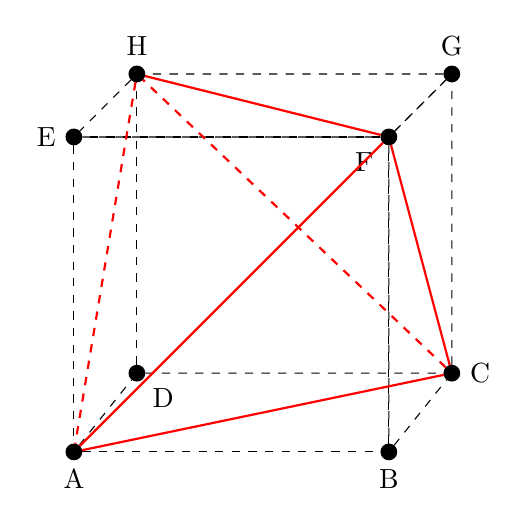
\begin{tikzpicture}
\foreach \n/\x/\l/\p in{
1/{( 0  , 0)}/{A}/below,
2/{( 4, 0)}/{B}/below,
3/{( .8, 1)}/{D}/south east,
4/{( 4.8, 1)}/{C}/right,
5/{( 0, 4)}/{E}/left,
6/{( 4, 4)}/{F}/south west,
7/{( 0.8, 4.8)}/{H}/above,
8/{( 4.8, 4.8)}/{G}/above
}
{
        \node[inner sep=2pt,circle,draw,fill,label={\p:\l}] (\n) at \x {};
    }
\draw[dashed] (1) -- (2) -- (6) -- (5) -- (1);
\draw[dashed] (5) -- (6) -- (8) -- (7) -- (5);
\draw[dashed] (2) -- (4) -- (8) -- (6) -- (2);
\draw[dashed] (1) -- (3) -- (4);
\draw[dashed] (3) -- (7);
\draw[thick, red,dashed] (4) -- (7) -- (1);
\draw[thick, red] (1) -- (4) -- (6) -- (7) -- (6) -- (1);
\end{tikzpicture}

\begin{tabular}{ | l | p{8cm} | l | l |}
    \hline
    type & description & example & \# \\
    \hline
    (4, 0, 0, 0) & id & (A)(C)(F)(H) & 1 \\
    \hline
    (1, 0, 1, 0) & rotation $2\pi/3$ around the axis between a point and the altitude to the opposing triangle & (A)(CFH) & 4 \\
    \hline
    (1, 0, 1, 0) & rotation $-2\pi/3$ around the axis between a point and the altitude to the opposing triangle & (A)(CHF) & 4 \\
    \hline
    (0, 2, 0, 0) & rotation around the axis between the centre of a line and the centre of the opposing segment & (AC)(HF) & 3 \\
    \hline
\end{tabular}

\text{}\newline

Total: 12.

\section{Even permutations}

\textbf{Note}

Composition is performed from the right.

\textbf{Lemma 1}

Any 3-cycle can be composed from 3-cycles of the form $(1, i, j)$.

\textbf{Proof}

For 3-cycles without $1$: $(a, b, c)$, this is trivially $(1, a, b)(1, b, c)$. For 3-cycles with 1: $(a, b, 1)$ we already have a solution.

\textbf{Lemma 2}

Any 3-cycle can be composed from 3-cycles of the form $(1, 2, j)$.

\textbf{Proof}

If the 3-cycle contains consecutively $1$ and $2$, then we are done. If it contains consecutively $2$ and $1$: $(a, 2, 1)$, then we apply the 3-cycle twice: $(a, 2, 1) = (1, 2, a)(1, 2, a)$.

If the 3-cycle contains $2$, but not $1$, then we simply apply Lemma 1. If the resulting 3-cycles contain $1, 2$ consecutivelly, then ok. If not, we can break them down again using applying the 3-cycle twice as previously.

If the 3-cycle contains $1$ and not $2$, then $(1, a, b) = (1, 2, b)(1, 2, b)(1, 2, a)(1, 2, b)$ and from Lemma 1 we can construct any 3-cycle of this form.

\textbf{Lemma 3}

$A_n$ is generated by 3-cycles of the form $(i, i+1, i+2)$.

\textbf{Proof}

From Lemma 2 we known, that any 3-cycle can be composed of more elementary cycles of the form $(1, 2, k)$. For $A_3 = \{ (1), (1, 2, 3), (1, 3, 2) \}$ we need only the generator $(1, 2, 3)$. For $A_4$ this is also true (checked programmatically by exhaustive state search). For $n \ge 5$: $(1, 2, i)$ it is obvious for $i = 3$ and for $i = 4$ it is also true, because $(1, 2, 4) = (1, 2, 3)(1, 2, 3)(2, 3, 4)(1, 2, 3)$.

For $i\ge 5$: $(1, 2, i)$ $= (1, 2, i-2)(1, 2, i -1)(i-2, i-1, i)(1, 2, i-2)(1, 2, i-1)$. From Lemma 2 we know, that any 3-cycle can be create by the product of 3-cycles of the form $(1, 2, j)$ and from the lecture we know, that any $A_k$ is generated by 3-cycles.


\textbf{Theorem}

Since we can use $\sigma = (1, 2, 3, \ldots, n)$, we can also use $\sigma^{-1} = \sigma^{n-1}$. Since we have $\alpha = (1, n-1, n)$, we can also use $(1, 2, 3) =\ ^{\sigma^2}\hspace{-0.2cm}\alpha$. This was we can create arbitrary cycle of the form $(i, i+1, i+2) = \ ^{\sigma^{1+i}}\hspace{-0.2cm}\alpha$. From Lemma 3 we know, that 3-cycles of the form $(i, i+1, i+2)$ generate $A_n$, so it can be also generated from $\alpha, \sigma$.

\end{document}
